\newpage
\chapter{Implementation}

\section{System Implementation}
The Mitsuketa system is implemented as a modular Python backend with a React frontend. The project directory is organized as follows:
\begin{itemize}
  \item \texttt{main.py} -- FastAPI application entry point with all REST API endpoints.
  \item \texttt{audio\_fingerprint.py} -- Audio signal processing and constellation map hash generation.
  \item \texttt{video\_fingerprint.py} -- Video keyframe extraction and pHash computation.
  \item \texttt{matcher.py} -- Fingerprint query, temporal alignment scoring, and BK-Tree search.
  \item \texttt{database.py} -- PostgreSQL connection management (psycopg2), schema creation, and batch I/O operations.
  \item \texttt{frontend/} -- React/Vite single-page application source.
\end{itemize}

\section{Experiment/Implementation Parameters}
\begin{table}[h!]
\centering
\caption{Key System Parameters}
\label{tab:params}
\begin{tabular}{p{5cm} p{3cm} p{5cm}}
\noalign{\hrule height 0.5mm}
\textbf{Parameter} & \textbf{Value} & \textbf{Description} \\
\hline
STFT Window Size & 4096 samples & Size of the FFT window for spectrogram generation \\
STFT Hop Length & 512 samples & Step size between successive STFT frames \\
Peak Neighborhood Size & $20 \times 20$ & Local neighborhood for spectrogram peak detection \\
Fan-Out Zone & 15 target peaks & Number of target peaks per anchor peak \\
Audio Confidence Threshold & 35\% & Minimum audio confidence for audio-only match \\
pHash Resolution & $32 \times 32$ px & Input frame size before DCT \\
pHash Length & 64 bits & Output perceptual hash length \\
BK-Tree Hamming Threshold & 10 bits & Max Hamming distance for a video match \\
DB Batch Insert Size & 5000 hashes & Number of hashes per batch PostgreSQL insert \\
DB Chunked Read Size & 50000 hashes & Number of hashes per read during matching \\
\noalign{\hrule height 0.5mm}
\end{tabular}
\end{table}

\section{User Interface}
The frontend is a React/Vite Single-Page Application styled with a Glassmorphism dark-mode theme. Key UI components include:
\begin{itemize}
  \item \textbf{Register Media Panel:} Drag-and-drop file upload with title input. Sends a \texttt{multipart/form-data} \texttt{POST} request to \texttt{/register}.
  \item \textbf{Identify Clip Panel:} Drag-and-drop clip upload with a progress indicator and real-time status messages (e.g., ``Extracting features...'', ``Matching hashes...'').
  \item \textbf{Results Panel:} Displays the matched title, confidence percentage (with a color-coded confidence bar), and a collapsible technical analysis log.
  \item \textbf{Library Panel:} Lists all registered media titles with their type (audio/video) and registration timestamp.
\end{itemize}

\section{Data Description}
The PostgreSQL database contains four core tables:

\begin{itemize}
  \item \textbf{\texttt{users}:} Manages authentication, hashed passwords, and Role-Based Access Control (RBAC) levels (Admin, Moderator, Viewer).
  \item \textbf{\texttt{media}:} Stores metadata (title, type, file path, duration) for each registered media item.
  \item \textbf{\texttt{audio\_fingerprints}:} Stores millions of constellation map hashes. Each row contains a \texttt{media\_id} (foreign key), a \texttt{fingerprint\_hash} (20-char truncated SHA-1), and a \texttt{time\_offset} (the anchor peak's absolute time in seconds).
  \item \textbf{\texttt{video\_fingerprints}:} Stores pHash strings for each keyframe. Each row contains a \texttt{media\_id}, a \texttt{frame\_index}, and a 64-bit \texttt{phash} stored as a 16-character hex string.
\end{itemize}

Advanced PostgreSQL indexing and connection pooling allow safe, highly concurrent reads and batch writes during media registration.

\section{Functional Implementation}

\subsection*{Audio Fingerprinting (\texttt{audio\_fingerprint.py})}
Audio is ingested via an FFmpeg subprocess piped directly to NumPy. The \texttt{librosa} library is used to generate the STFT-based spectrogram. Peak detection uses a local maximum filter over a $20 \times 20$ neighborhood. The fan-out loop (pairing each anchor with up to 15 targets) is JIT-compiled using \textbf{Numba} for significant speedup on large files.

\subsection*{Video Fingerprinting (\texttt{video\_fingerprint.py})}
FFmpeg extracts one keyframe every two seconds. Each frame is passed to the \texttt{ImageHash} library's \texttt{phash()} function, which internally performs the grayscale resize and DCT computation. The resulting hash object is stored as a hex string.

\subsection*{Matching Engine (\texttt{matcher.py})}
The audio matching function reads fingerprints from the database in configurable chunks (50,000 hashes at a time) to avoid memory overflow for large libraries. A Python \texttt{collections.Counter} tallies temporal offsets ($\Delta t$) for each candidate media ID. The candidate with the highest aligned count is returned. For video, the BK-Tree (built from all stored pHashes using \texttt{pybktree}) is queried with a threshold of 10, and the media ID with the highest match count wins.

\section{Output}
The system returns a JSON response to the frontend with the following structure:
\begin{verbatim}
{
  "match_found": true,
  "title": "Interstellar Official Trailer",
  "confidence": 87.4,
  "match_type": "audio",
  "audio_hashes_matched": 312,
  "audio_hashes_total": 357,
  "video_hashes_matched": 0,
  "analysis_log": [
    "Extracting audio fingerprints from query...",
    "Querying 1,247,832 audio hashes in database...",
    "Top candidate: 'Interstellar Official Trailer' (312 aligned matches)",
    "Audio confidence: 87.4% -- STRONG MATCH"
  ]
}
\end{verbatim}

\section{System UI Screenshots}
The following screenshots demonstrate the working flow of the React/Vite single-page application, showing the authentication screens, dashboard, library, and active identification processes.

\begin{figure}[h!]
  \centering
  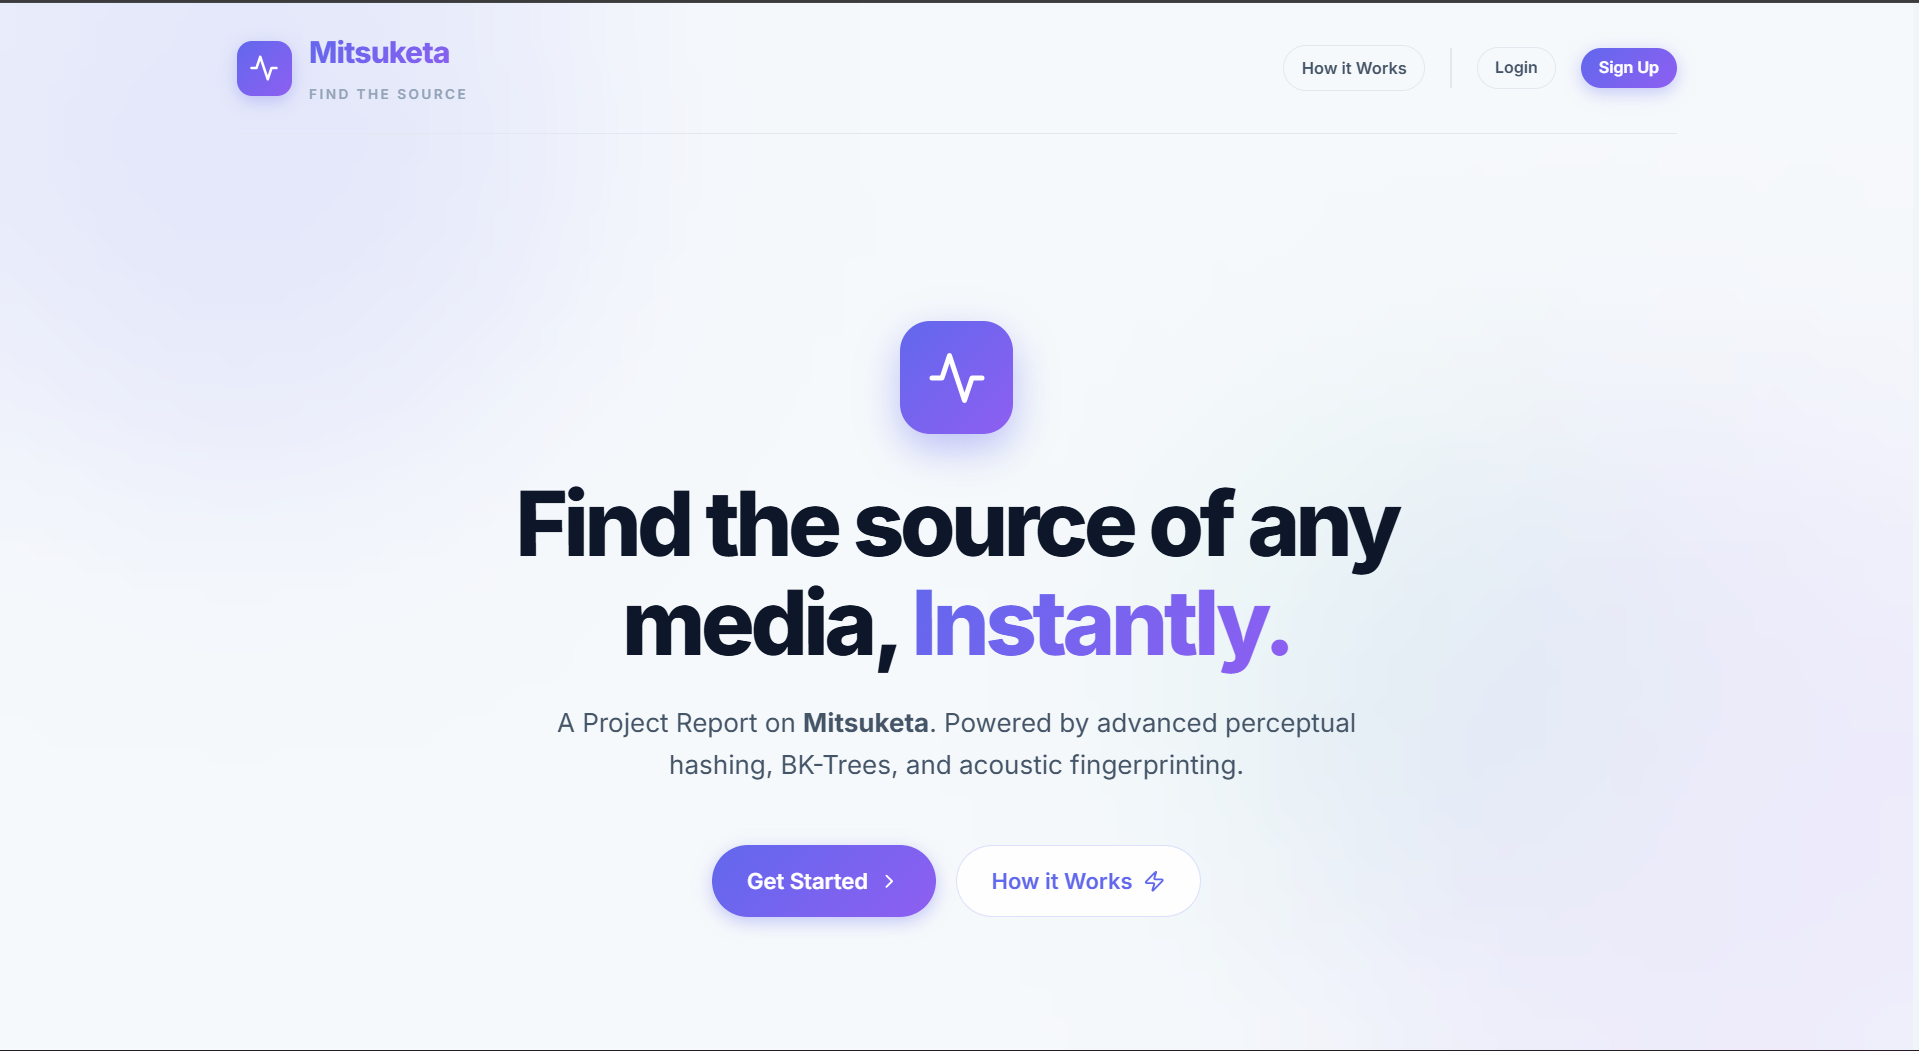
\includegraphics[width=0.8\textwidth]{ui_screenshot_1}
  \caption{Mitsuketa User Interface - View 1}\label{fig:ui1}
\end{figure}

\begin{figure}[h!]
  \centering
  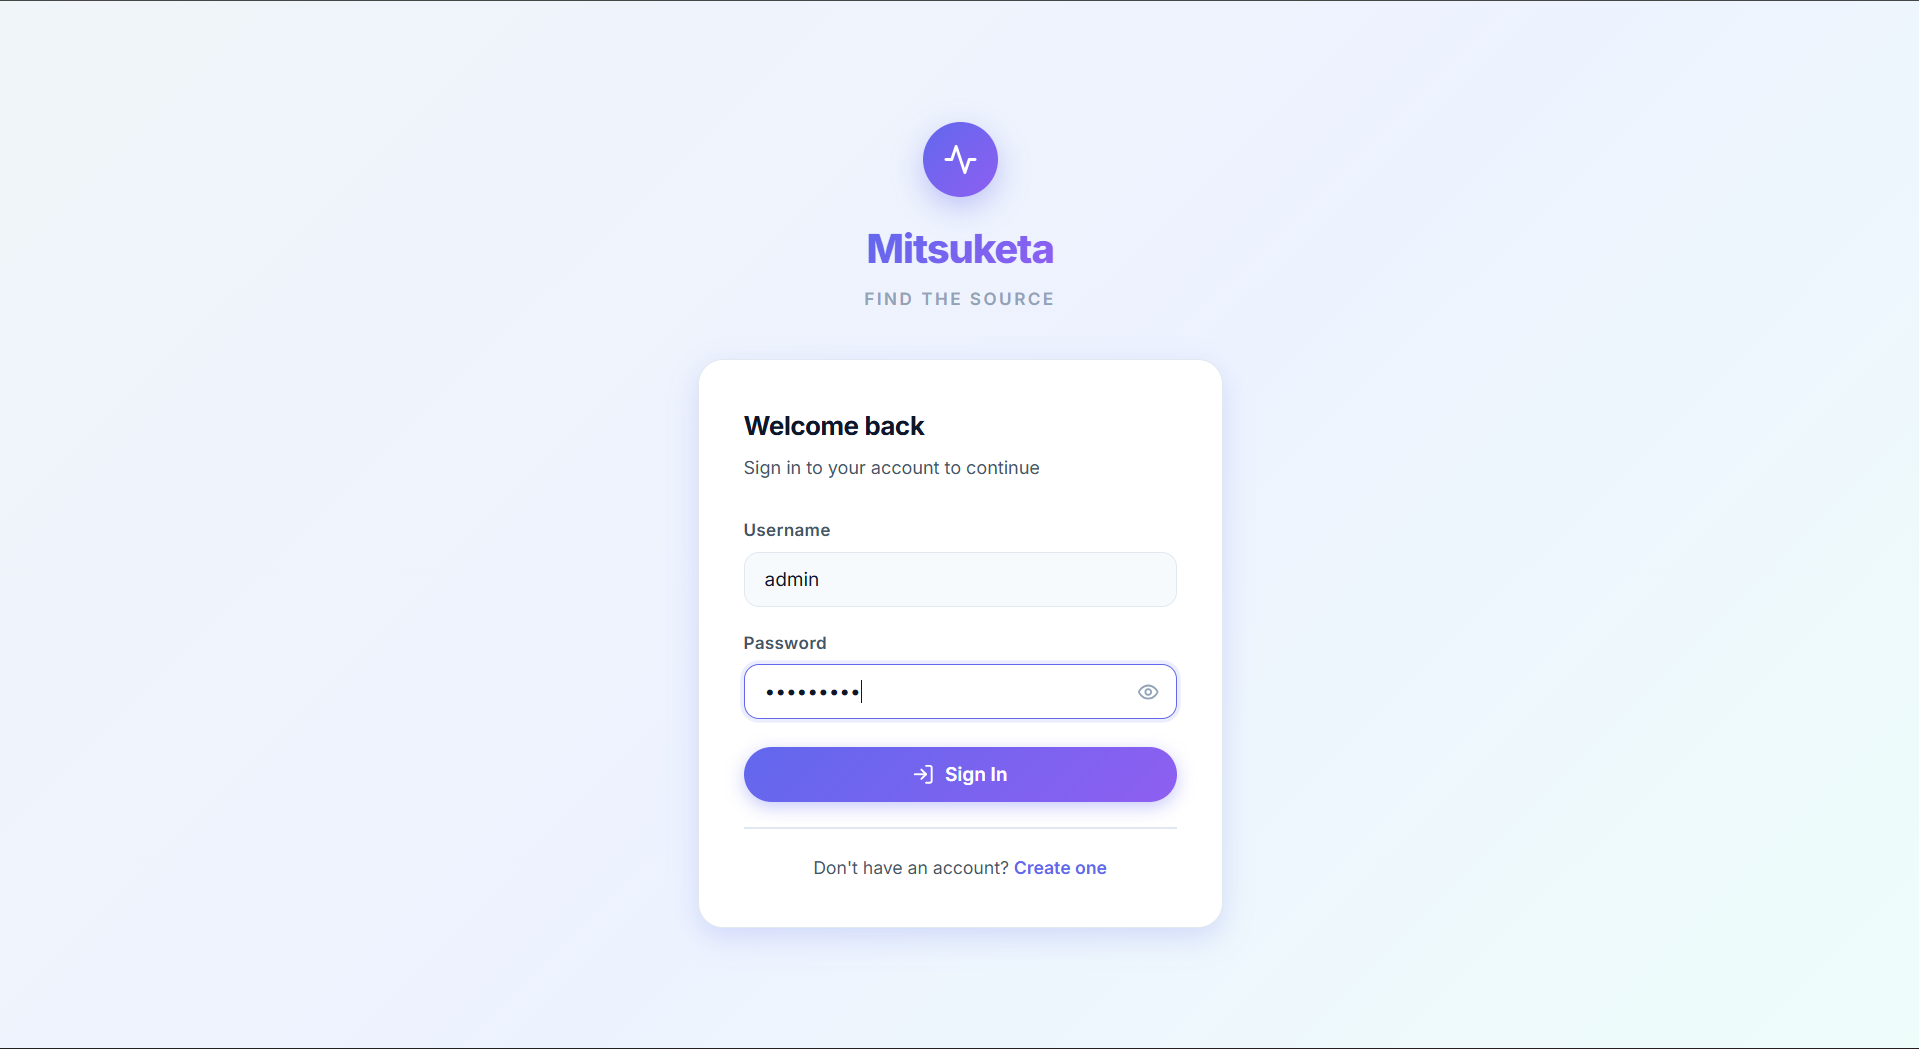
\includegraphics[width=0.8\textwidth]{ui_screenshot_2}
  \caption{Mitsuketa User Interface - View 2}\label{fig:ui2}
\end{figure}

\begin{figure}[h!]
  \centering
  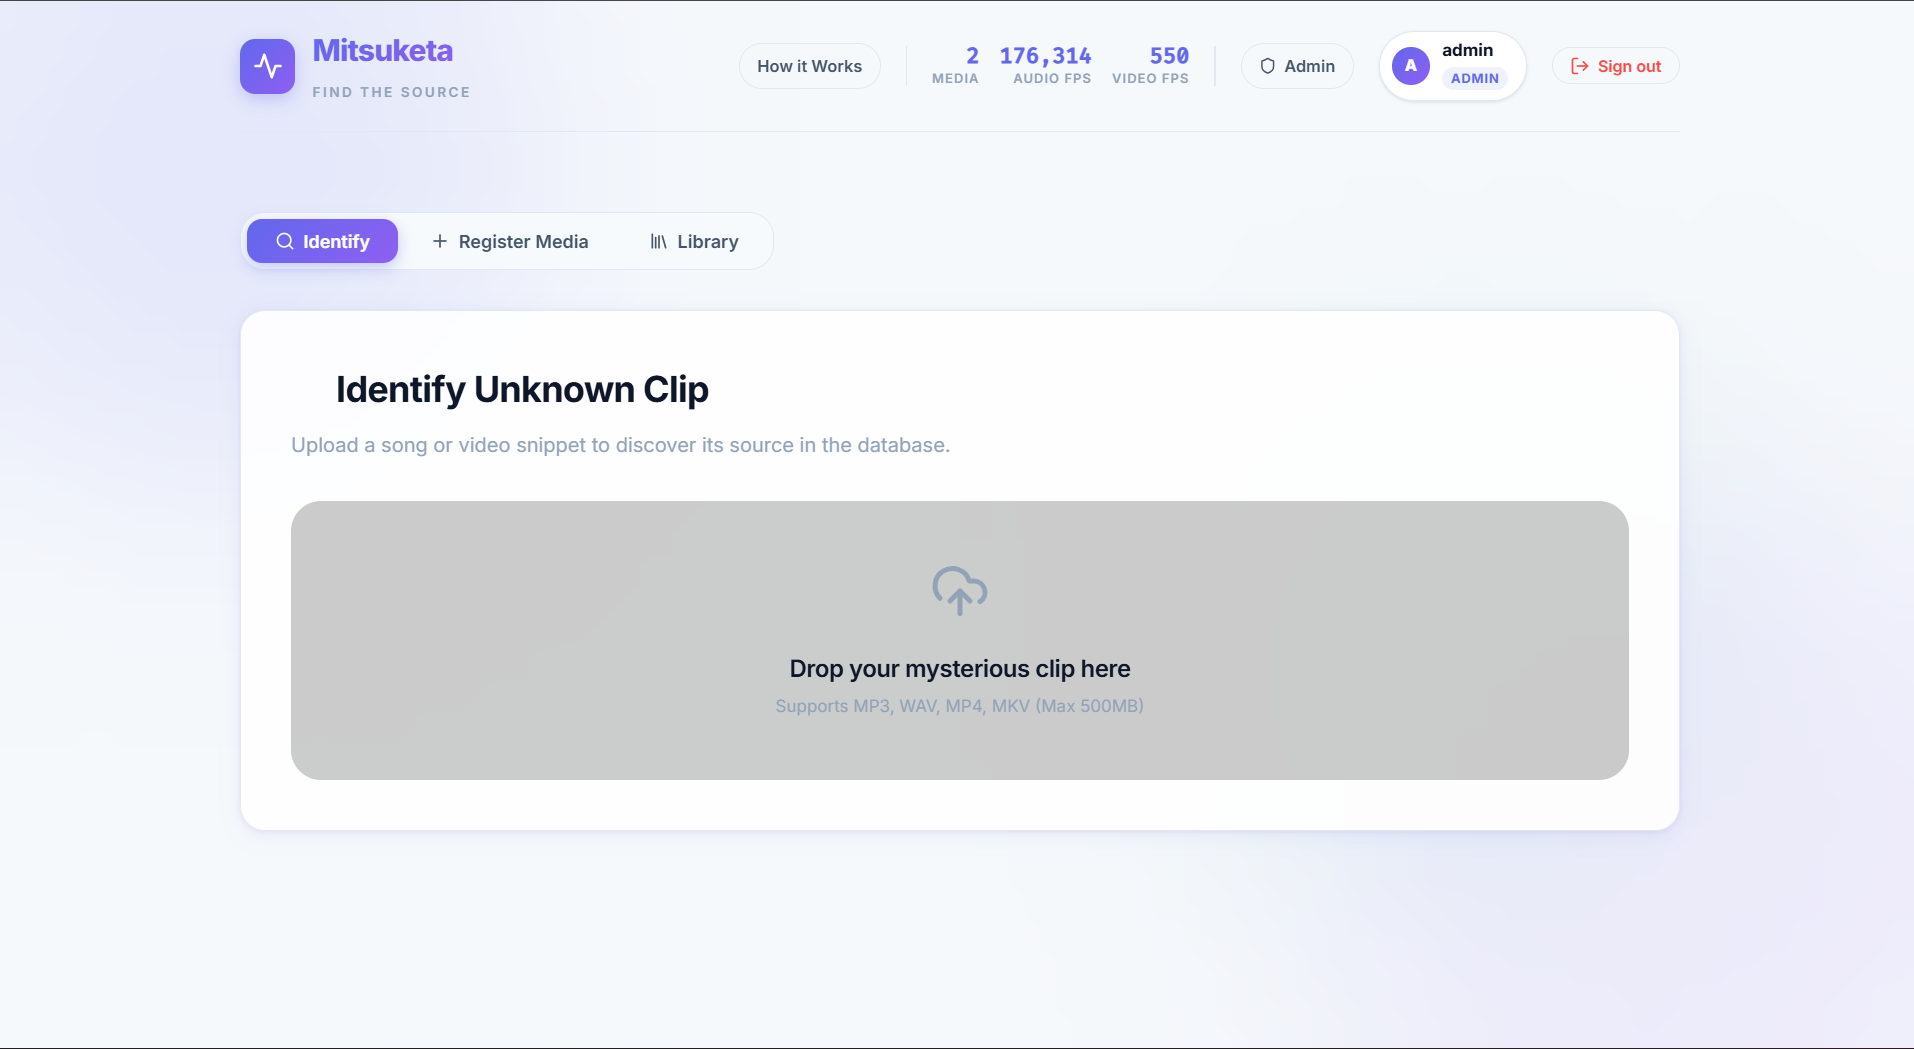
\includegraphics[width=0.8\textwidth]{ui_screenshot_3}
  \caption{Mitsuketa User Interface - View 3}\label{fig:ui3}
\end{figure}

\begin{figure}[h!]
  \centering
  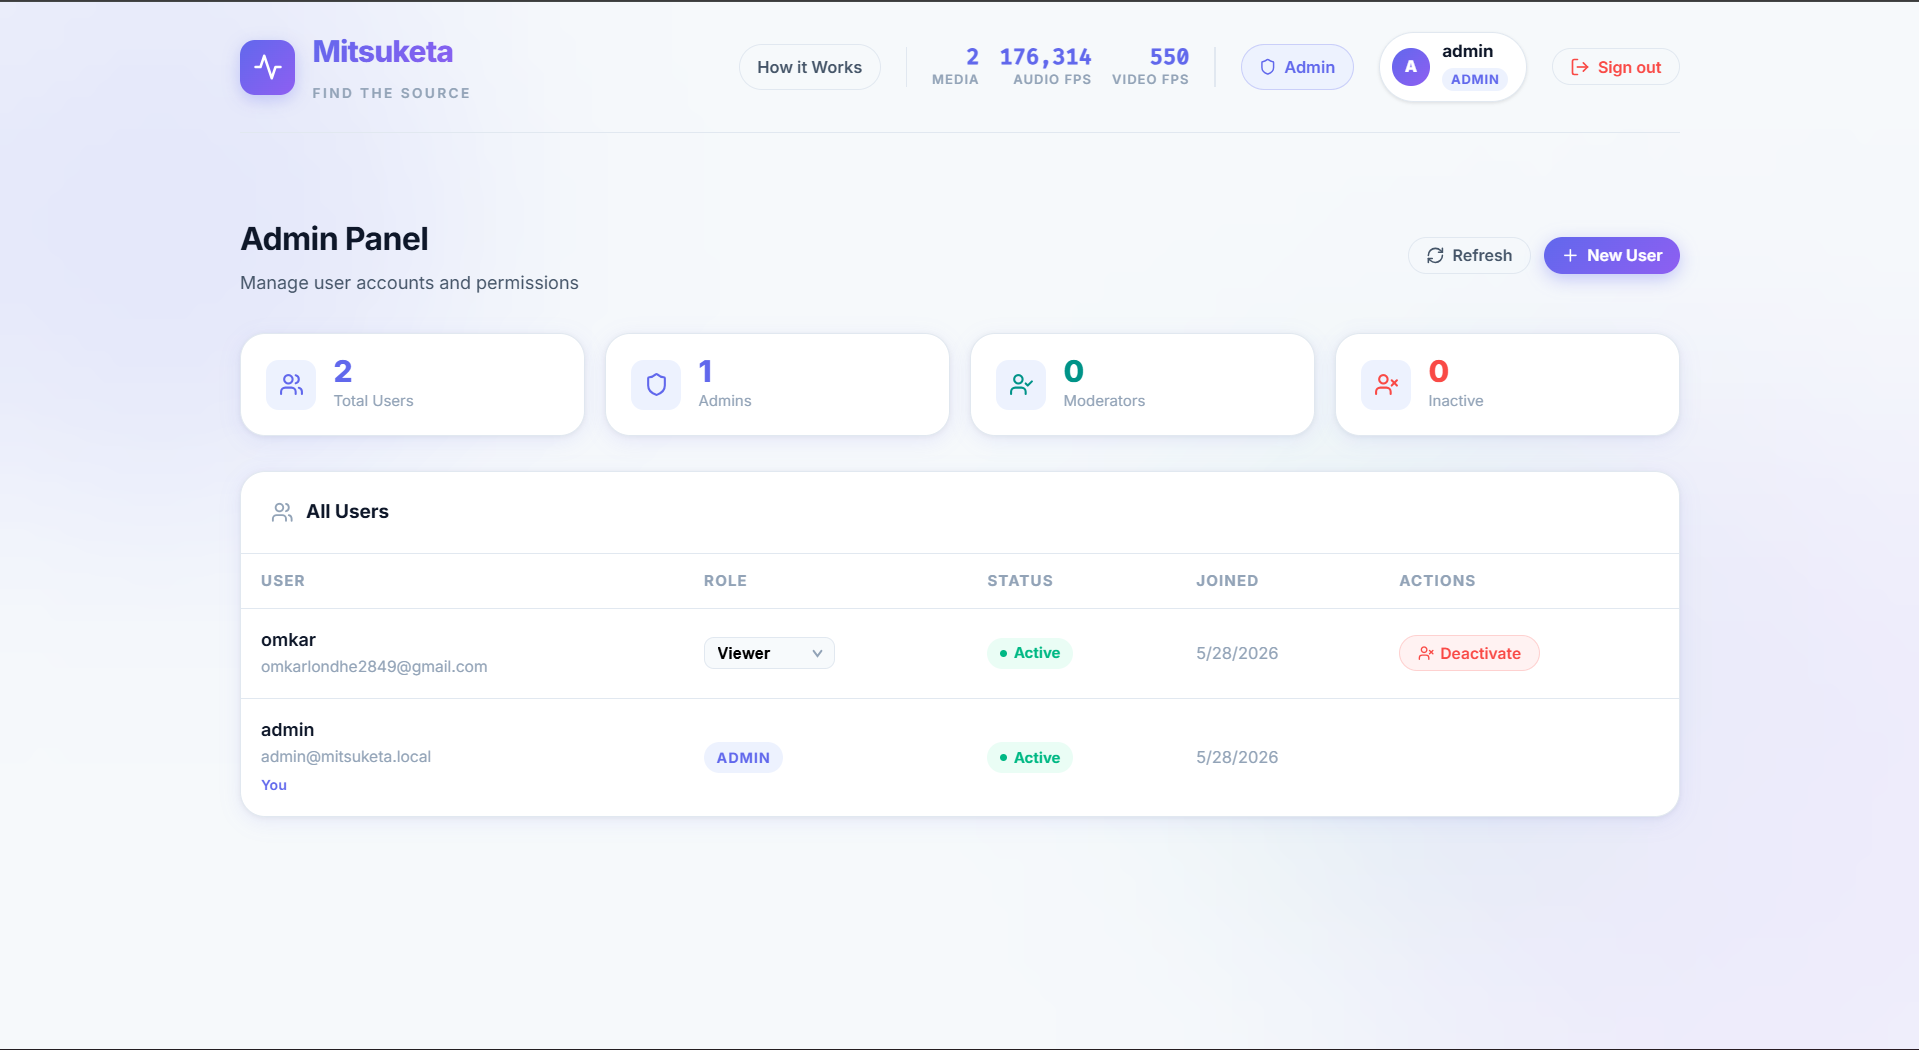
\includegraphics[width=0.8\textwidth]{ui_screenshot_4}
  \caption{Mitsuketa User Interface - View 4}\label{fig:ui4}
\end{figure}

\begin{figure}[h!]
  \centering
  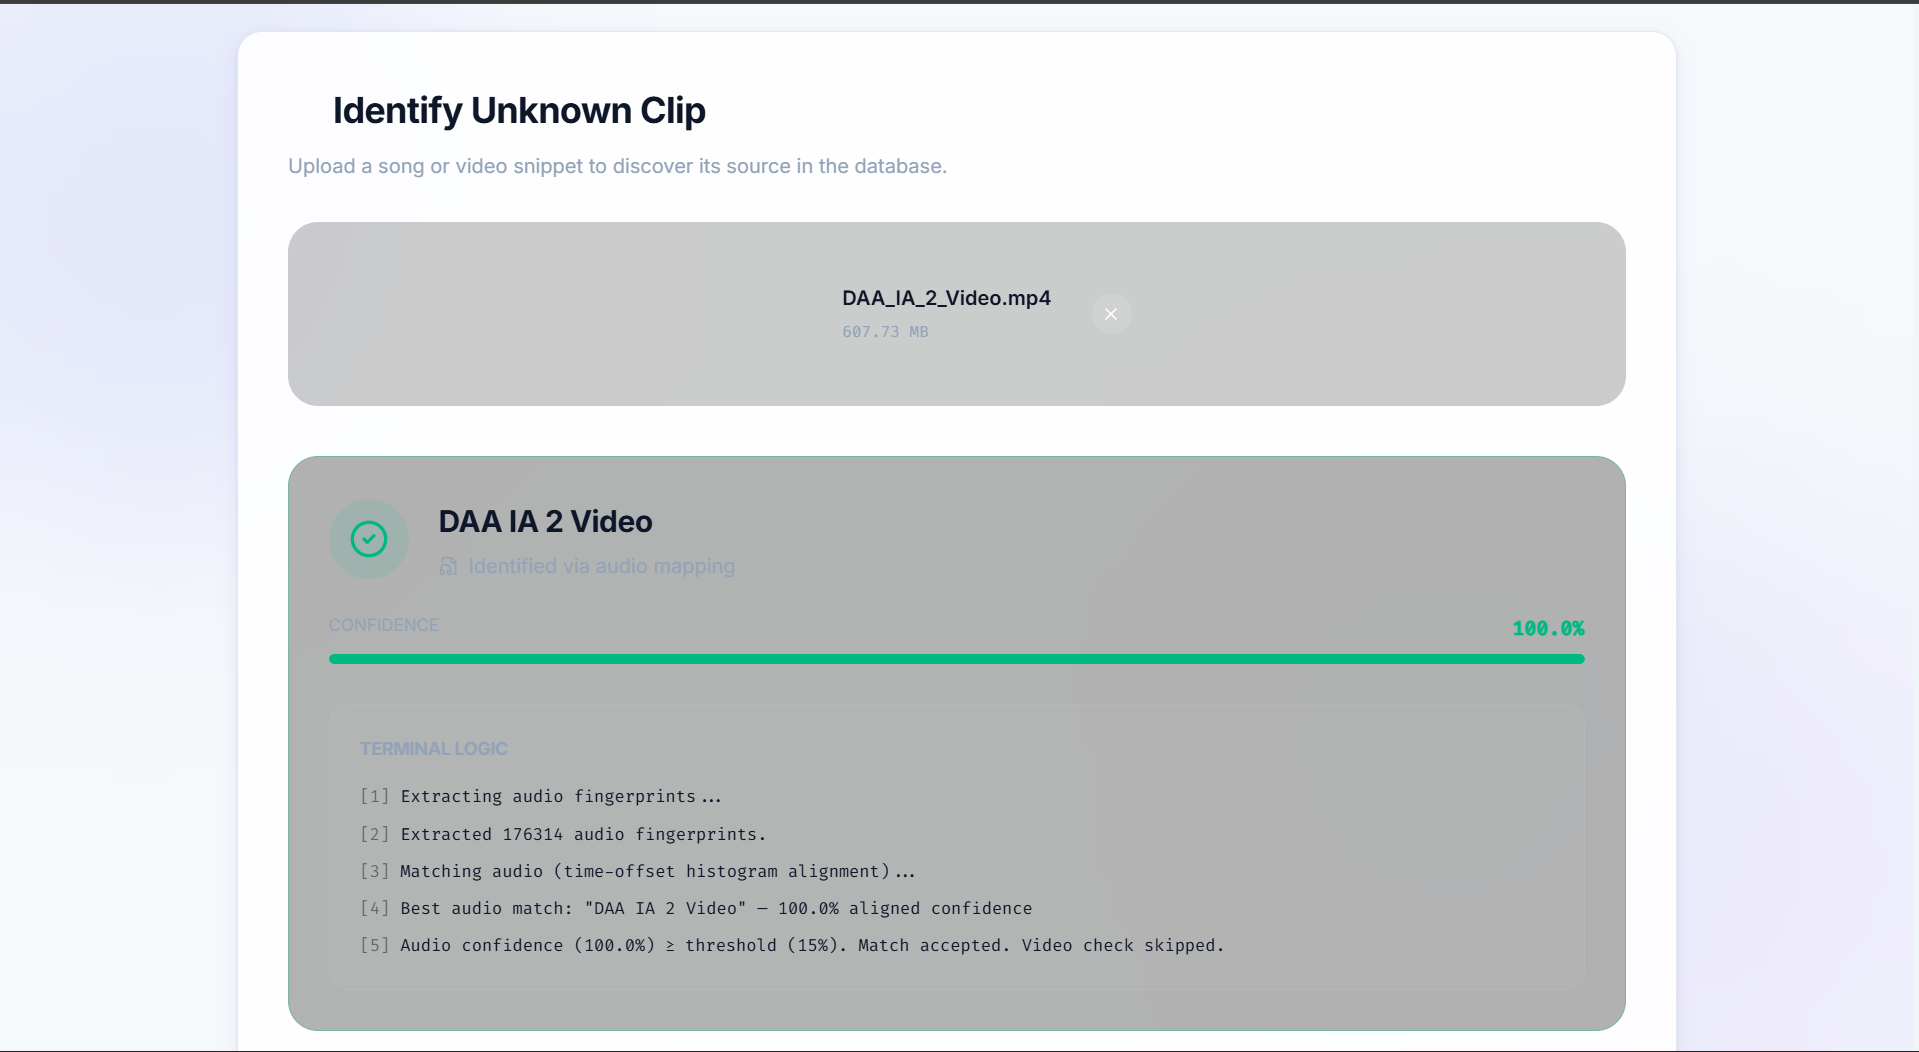
\includegraphics[width=0.8\textwidth]{ui_screenshot_5}
  \caption{Mitsuketa User Interface - View 5}\label{fig:ui5}
\end{figure}

\begin{figure}[h!]
  \centering
  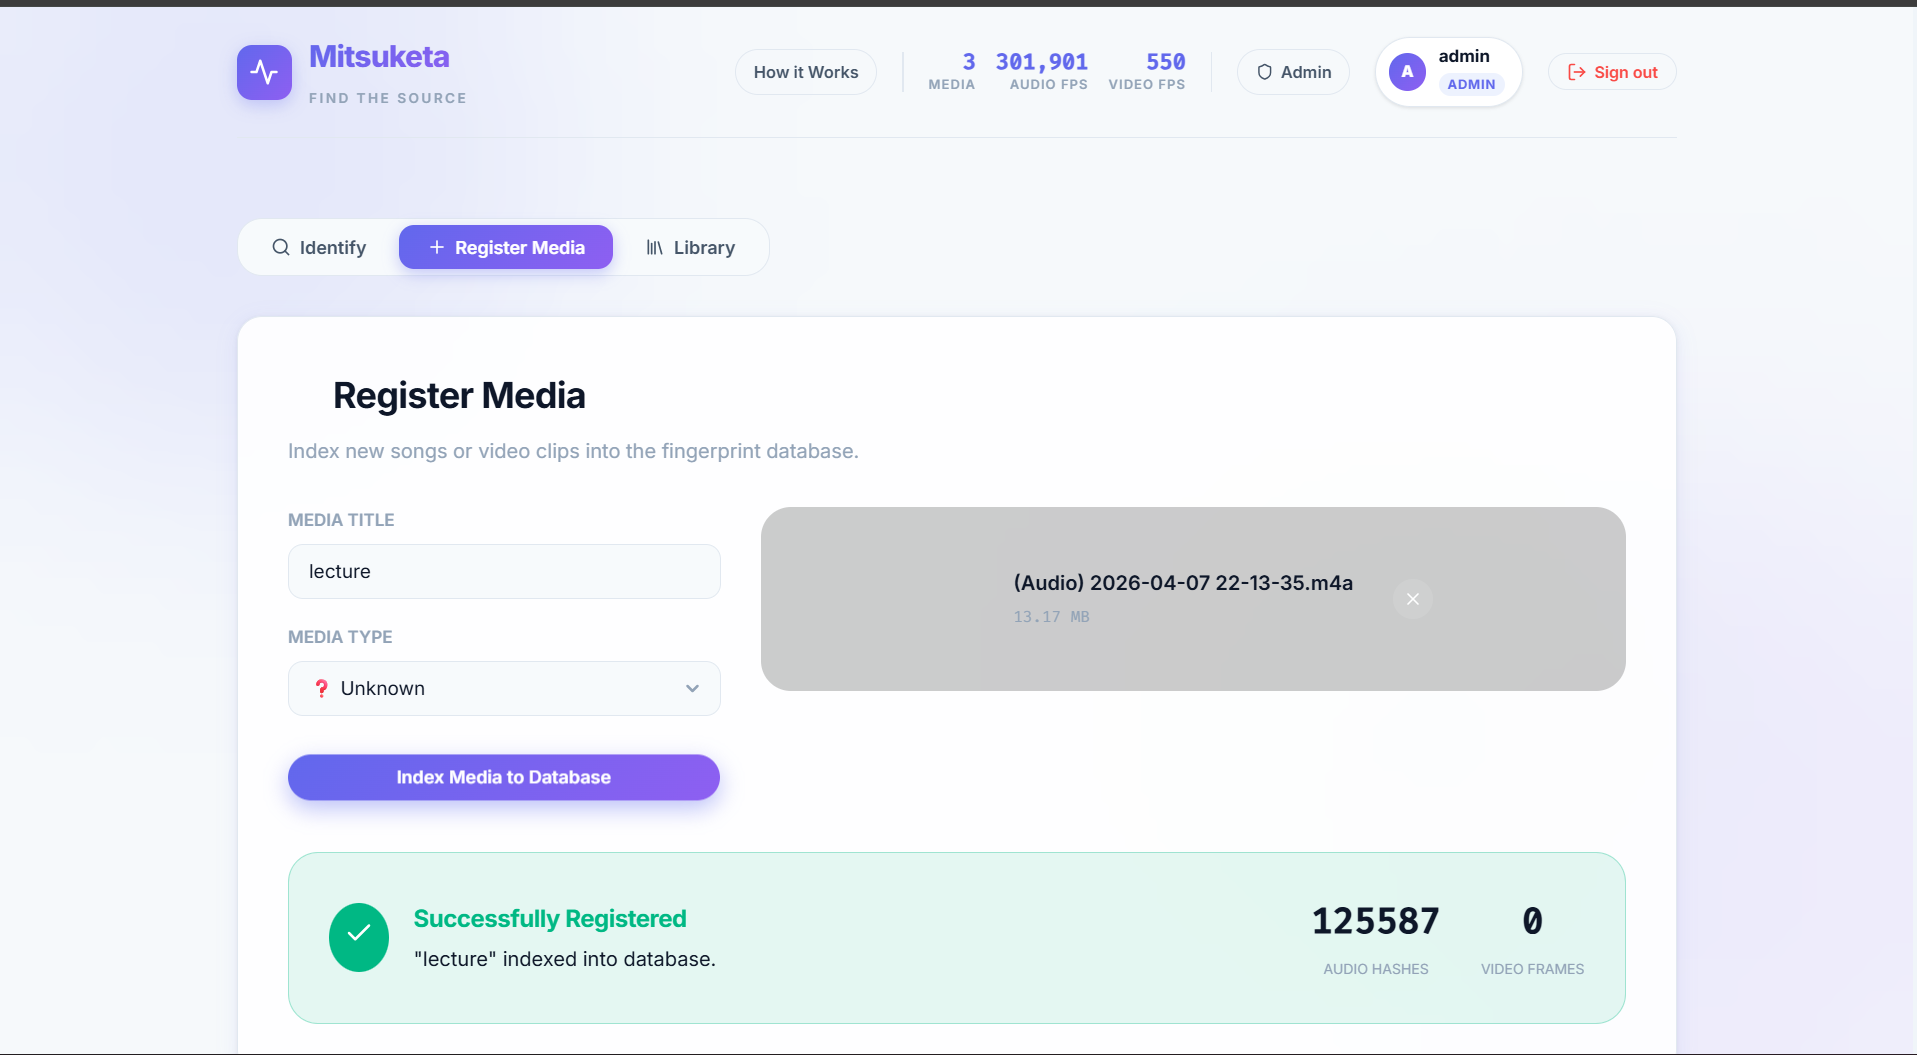
\includegraphics[width=0.8\textwidth]{ui_screenshot_6}
  \caption{Mitsuketa User Interface - View 6}\label{fig:ui6}
\end{figure}

\begin{figure}[h!]
  \centering
  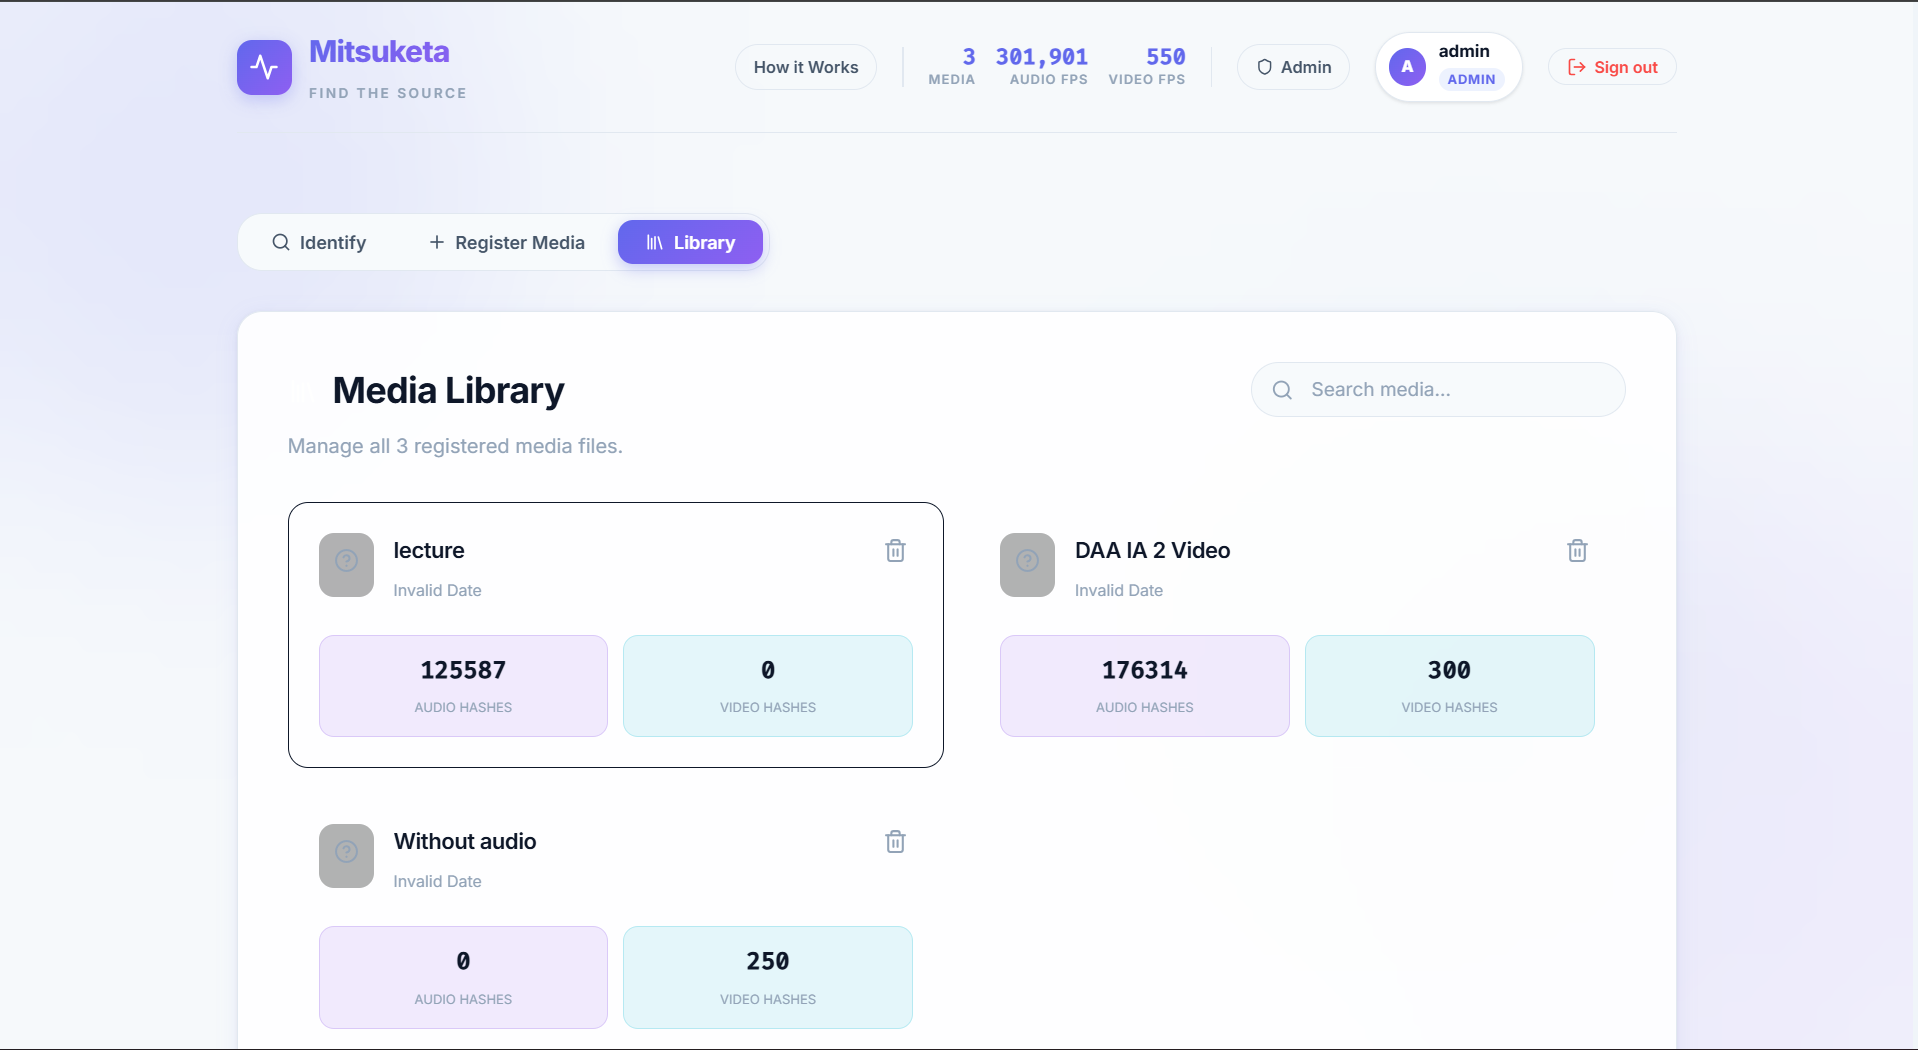
\includegraphics[width=0.8\textwidth]{ui_screenshot_7}
  \caption{Mitsuketa User Interface - View 7}\label{fig:ui7}
\end{figure}

\begin{figure}[h!]
  \centering
  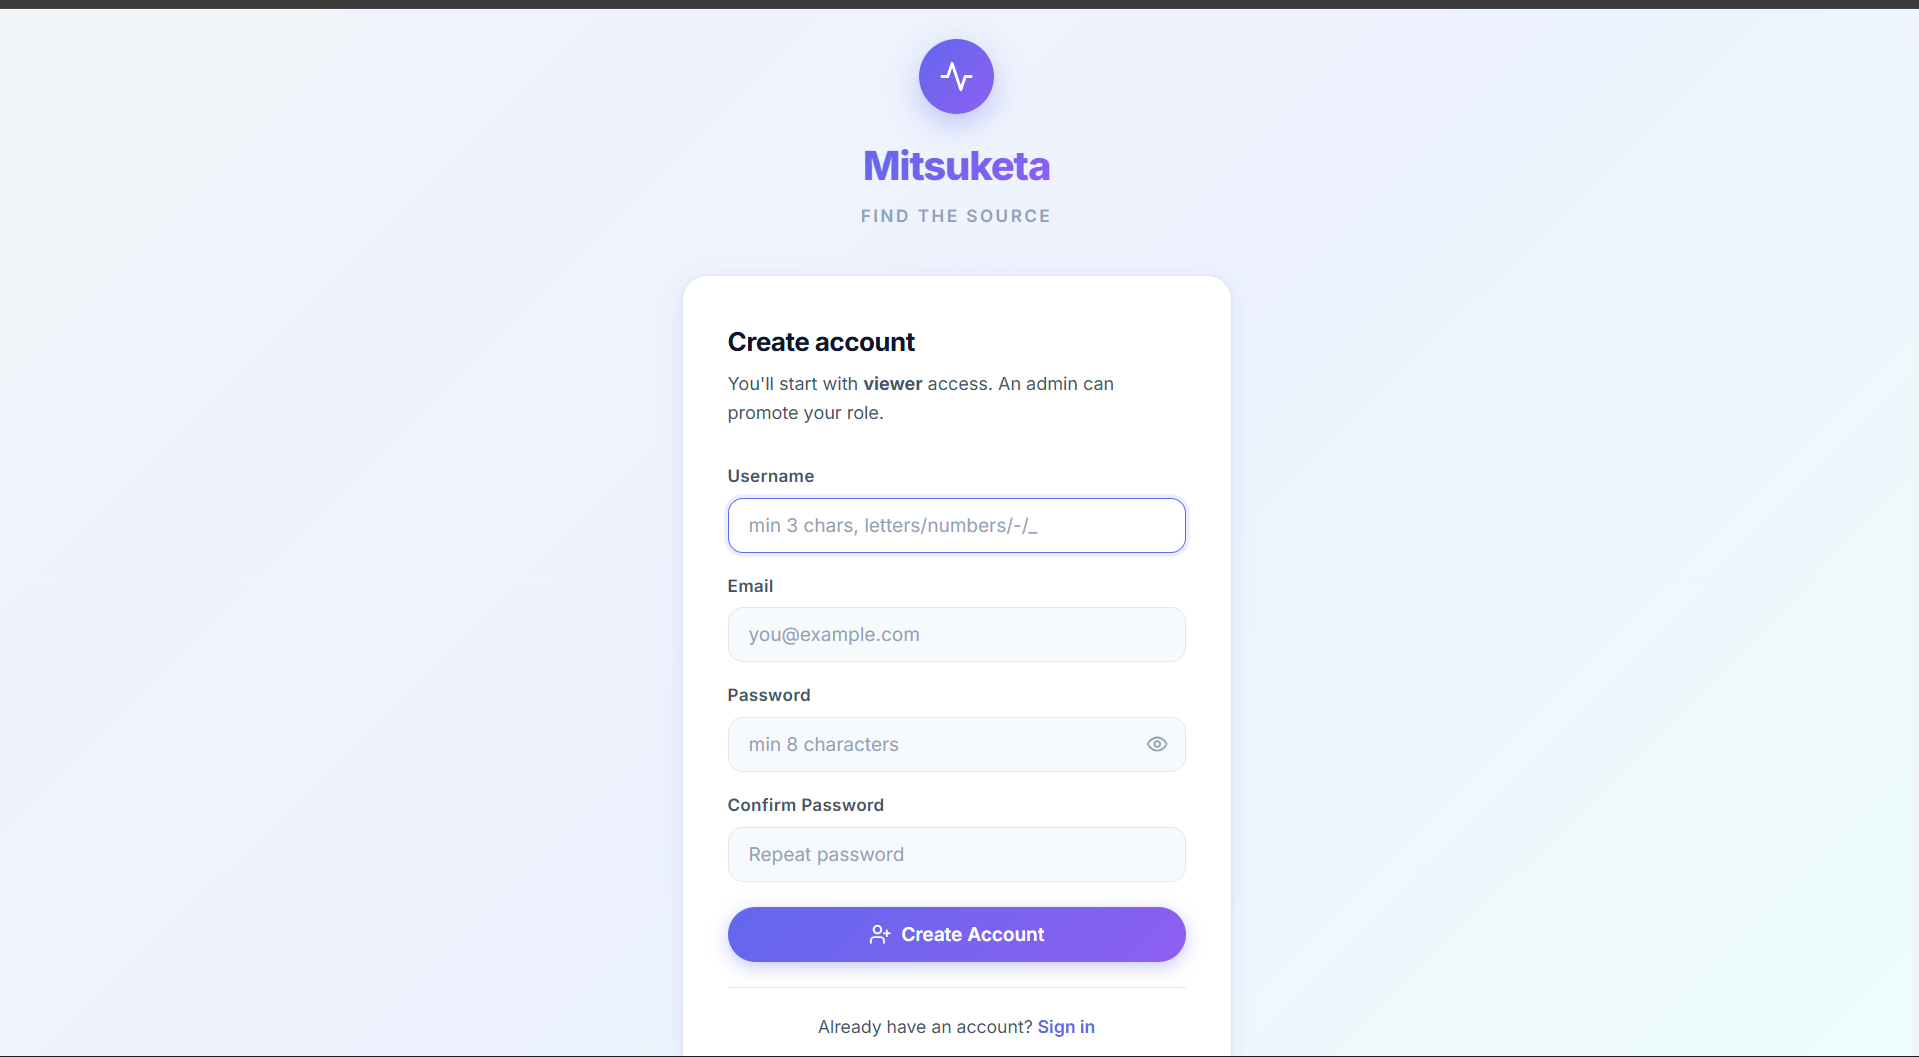
\includegraphics[width=0.8\textwidth]{ui_screenshot_8}
  \caption{Mitsuketa User Interface - View 8}\label{fig:ui8}
\end{figure}

\begin{figure}[h!]
  \centering
  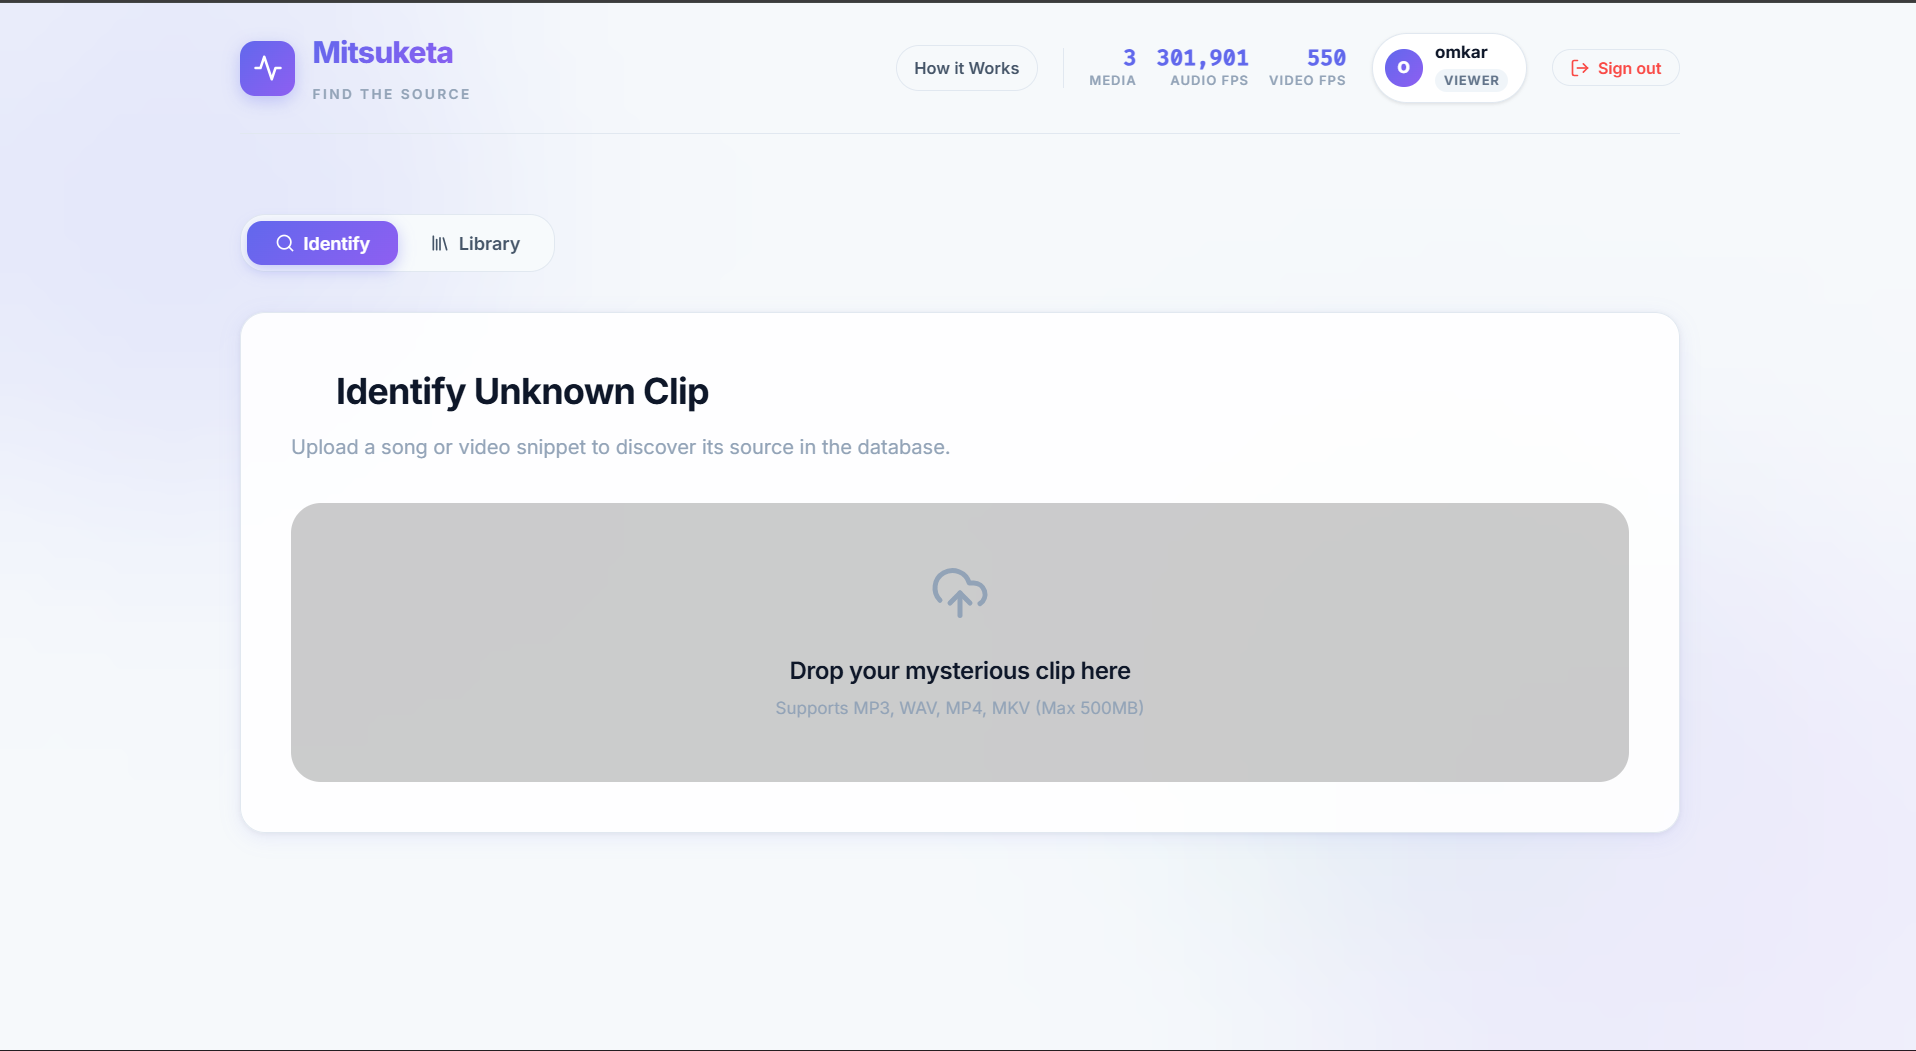
\includegraphics[width=0.8\textwidth]{ui_screenshot_9}
  \caption{Mitsuketa User Interface - View 9}\label{fig:ui9}
\end{figure}

\vspace{10mm}
\hrule